\section{Construction}\label{sec:construction}

\subsection{The Setting}

We are given $n$ DLPs $\wheel[1], \wheel[2], \ldots, \wheel[n]$. These are preexisting, already operational
DLPs such as Bitcoin, Ethereum, and Cardano. Our goal is to build a \emph{new} DLP $\RB$
on top of these such that, if the majority of \emph{underlying}
$\wheel[1], \ldots, \wheel[n]$ are \emph{secure}, then so is the
\emph{overlay} DLP $\RB$. As $\RB$ is a DLP, it will have its own population of $m$ nodes
$\RB_1, \RB_2, \ldots, \RB_m$. The $\RB$ DLP will have its own type of transaction and a
ledger consisting of these transactions. For example, it can maintain its own coin\footnote{
We will not be concerned with bridging this coin from the overlay ledger to the underlying
ledgers. This can be done using various standard bridging techniques which are orthogonal
to this work~\cite{pow-sidechains,pos-sidechains,zkbridge}.}. Importantly, similarly to
a rollup, \emph{we will not make any additional security assumptions about the honesty of the
$\RB$ nodes}.

\emph{Each} of these $\RB$ nodes runs a separate full node $\wheel[1], \ldots, \wheel[n]$ for each of
the underlying DLPs. The $\RB$ nodes do not have direct network communication, but only
use the read/write functionalities of their respectie $\wheel[1], \ldots, \wheel[n]$ instances to communicate.
For example, when party $\RB[1]$ \emph{writes} a transaction $\tx$ to its $\wheel[1][1]$ instance,
this transaction will eventually appear in $\RB[2]$'s $\wheel[1][2]$ instance ledger output,
as long as $\wheel[1]$ is live.
We will use $\wheel[i][j][r]$ to refer to the ledger reported at round $r$ by the full node instance
running the underlying DLP $\wheel[i]$ operated by the overlay party $\RB[j]$
(this ledger, like all ledgers, is a sequence of transaction/timestamp pairs, and its
$k^\text{th}$ transaction/timesetamp pair is $\wheel[i][j][r][k]$).

\textbf{Bulletins.}
We do not want to modify the underlying DLPs to support our protocol. However, the underlying DLPs
do not understand the transaction semantics of our overlay ledger. We will therefore use the underlying
DLPs as a simple lazy transaction ordering service. We will assume that we can take any
arbitrary string $w$ and \emph{encode} it into a transaction suitable for each underlying ledger.
Such transactions are \emph{always} accepted by the underlying ledger, and their contents
are not validated (beyond checking that a minimum fee is suitably paid to avoid spamming attacks).
We call a DLP that supports writing such arbitrary data into it a \emph{bulletin}. A bulletin
DLP offers two additional functions $\tx \gets \textsf{encode}(s)$ and $s \gets \textsf{decode}(\tx)$.
The $\textsf{encode}$ function one takes a string $s$ and encodes it into a transaction $\tx$ that can be \emph{written}
into the DLP and is guaranteed to be accepted. The $\textsf{decode}$ function takes a transaction $\tx$
and, if it is a bulletin transaction, decode it back into $s$. Otherwise, $\textsf{decode}$ can return $\bot$.
All transactions produced by $\textsf{encode}$
are bulletin transactions, but the adversary can also introduce arbitrary bulletin transactions of her choice
indiscriminately.

\begin{definition}[Bulletin]
  A DLP $\Pi$ accompanied by a pair of functions $(\textsf{encode}, \textsf{decode})$,
  is called a \emph{bulletin}. It must hold that, for any $s \in \{0, 1\}^*$,
  the output of $\tx = \textsf{encode}(s)$ is always a valid
  transaction and that $\textsf{decode}(\textsf{encode}(s)) = s$.
\end{definition}

Bulletins can order and ensure data availability of arbitrary data without checking
any semantic validity. As such, they constitute a \emph{lazy} use of a ledger~\cite{lazyledger,lazylight}.

\subsection{A Majority Vote}\label{sec:construction-naive}

\import{./}{algorithms/alg-majorityvote}

\begin{figure*}
    \centering
    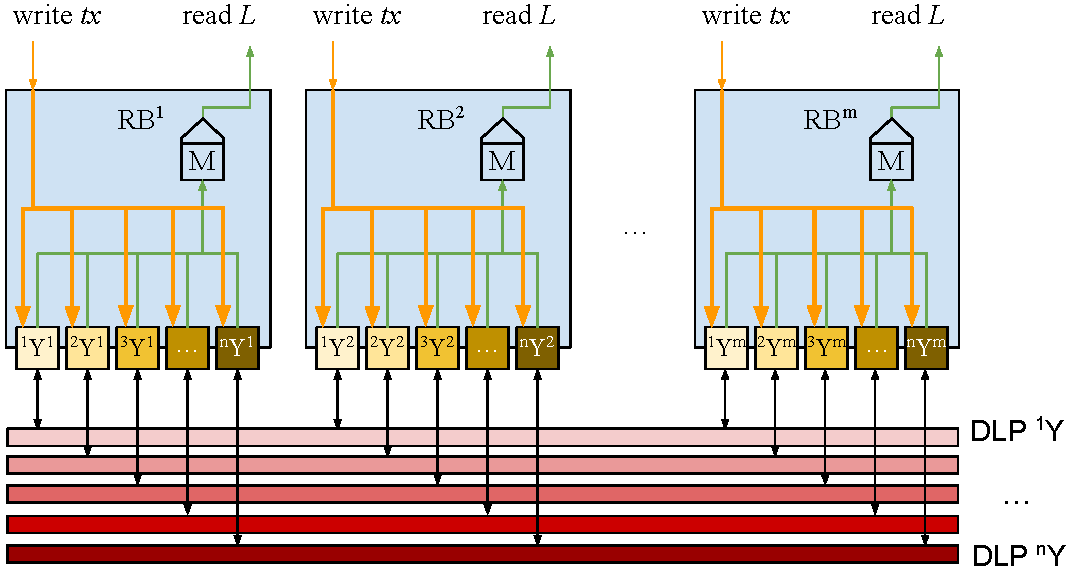
\includegraphics[width=\textwidth,keepaspectratio]{figures/rollerblade-naive-construction.pdf}
    \caption{The first attempt at the composed construction. Here,
             $m$ different parties $\RB_1, \ldots, \RB_m$ operate Rollerblade
             nodes, each of which runs a client on $n$ different underlying
             DLPs $Y_1, \ldots, Y_n$.}
    \label{fig.naive}
\end{figure*}

In Figure~\ref{fig.naive}, $m$ parties $\RB[1], \ldots, \RB[m]$ run the overlay protocol.
Each of the $\RB$ nodes runs
a full node to each of the $n$ underlying DLPs $\wheel[1], \ldots, \wheel[n]$, pictured as squares
of varying shades of yellow. The full nodes communicate with one another using their
respective DLP technology, which we treat as a black box here, depicted as elongated
rectangles in varying shades of red towards the bottom of the figure. The $\RB$ nodes
make their own overlay DLP, offering \emph{read} and \emph{write} functionalities.
When an $\RB$ transaction $\tx$ is \emph{written} into one of the $\RB$ nodes by the user,
the $\RB$ serializes this transaction for each of the underlying DLPs (using the
serialization mechanism particular to each individual DLP) and posts it
as a transaction there, depicted as orange wires running downwards. Each of the
full nodes then propagates this transaction using its own DLP technology to the
other full nodes. For example, if the underlying $\wheel[1]$ DLP is secure, then
the full node $\wheel[1][2]$ running within $\RB[2]$ will eventually see the transaction
posted by $\RB[1]$ into its own $Y[1][1]$ full node. When the $\RB$ user requests to read the
ledger of the respective $\RB$ node, the node invokes the respective \emph{read}
functionality of all of its full node boxes, depicted as green wires running upwards
in the figure. The output of this \emph{read} operation is then filtered and deserialized
(using the deserialization mechanism particular to each individual DLP), then fed into a
\emph{majority voting} contraption, denoted with the letter M and the \emph{house} symbol
in the figure, which then outputs the desired ledger $L$ of $\RB$ transactions (top).

\subsection{A BFT to Rule Them All}\label{sec:construction-bft}

\begin{itemize}
  \item Simple majority voting construction with no BFT protocol on top. Serialization and deserialization requirements and algorithms. Majority voting on ``ledger extensions'' algorithm. Fragile results in which different blockchains can disagree on the order and one blockchain can ``flip over'' the result. l. Condorcet cycles.
  \item The necessity of running a BFT protocol on top, but without talking about the oracle abstraction of signatures, broadcasting, verification, and receiving. Light clients from one blockchain to another using smart contracts. Using the blockchains as ports of communication.
  \item Oraclizing sign/broadcast and receive/verify.
  \item Remove the smart contract assumption using dirty ledgers.
  \item The full construction.
\end{itemize}

\subsection{Compatibility}\label{sec:compatibility}

\import{./}{algorithms/alg-rollerblade}
\import{./}{algorithms/alg-relay}
\import{./}{algorithms/alg-view}
\import{./}{algorithms/alg-simulate}
\import{./}{algorithms/alg-encode}
\import{./}{algorithms/alg-ledger}
